\documentclass[tikz,border=3pt]{standalone}
\usepackage{amsmath}
\usepackage{tikz}
\usepackage{pgfplots}
\pgfplotsset{compat=1.18}
\begin{document}
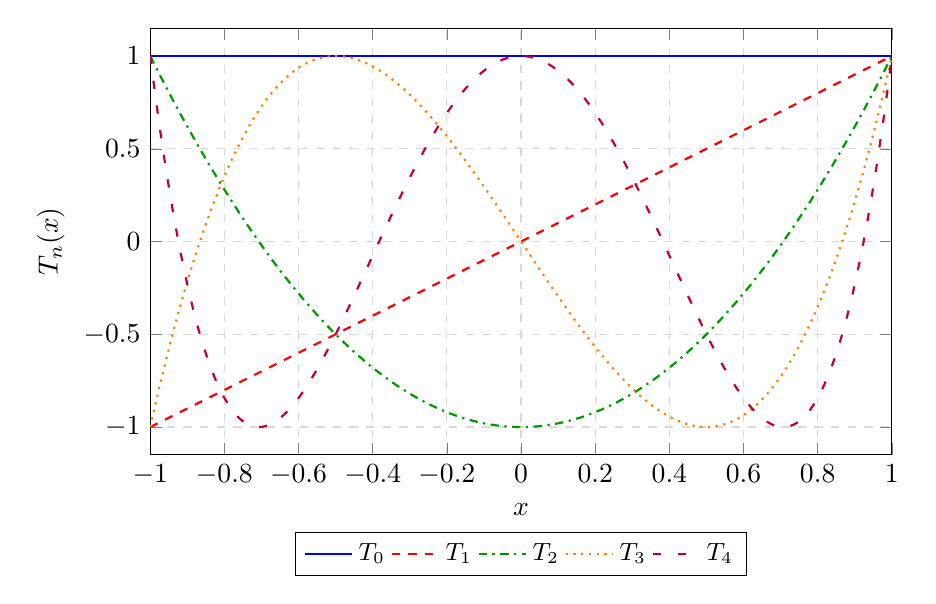
\begin{tikzpicture}
\begin{axis}[
  width=11cm, height=7cm,
  xlabel=$x$, ylabel={$T_n(x)$},
  xmin=-1, xmax=1, ymin=-1.15, ymax=1.15,
  legend style={at={(0.5,-0.18)}, anchor=north, font=\small},
  legend columns=5,
  grid=both, grid style={dashed, gray!30},
  domain=-1:1, samples=300,
  no marks
]
  \addplot[blue, thick, solid]           {1};
  \addlegendentry{$T_0$}
  \addplot[red, thick, dashed]            {x};
  \addlegendentry{$T_1$}
  \addplot[green!60!black, thick, dashdotted] {2*x^2 - 1};
  \addlegendentry{$T_2$}
  \addplot[orange, thick, dotted]         {4*x^3 - 3*x};
  \addlegendentry{$T_3$}
  \addplot[purple, thick, loosely dashed]         {8*x^4 - 8*x^2 + 1};
  \addlegendentry{$T_4$}
\end{axis}
\end{tikzpicture}
\end{document}
